% IMPORTANT: add or remove (comment out) the boolean '\solutiontrue' below to
% create the solution document or the exercise document respectively.
% First we create the switch to make either the exercises or the solutions
\newif\ifsolution\solutionfalse
% To create the solution uncomment '\solutiontrue'
\solutiontrue

\documentclass[a4paper,11pt]{article}
\title{System Security,
\ifsolution Solution \else \fi
Buffer Overflow 0}


\include{author}

\usepackage[T1]{fontenc}
\usepackage{ae, aecompl}
\usepackage{a4wide}
\usepackage{boxedminipage}
\usepackage{url}
\usepackage{graphicx}
\usepackage{enumerate}
\usepackage{alltt}
\usepackage{hyperref}
\usepackage{listings}
\usepackage{drawstack}
\usepackage{xcolor}

% Some useful commands and environments
\usepackage{framed}
\newenvironment{solution}%
{\par{\noindent\small\textit{Solution:}}\vspace{-12pt}\begin{framed}}%
{\end{framed}\par}



%% tty - for displaying TTY input and output
\newenvironment{tty}%
{\small\begin{alltt}}%
{\end{alltt}}

\begin{document}
\maketitle

This exercise session will help you to gain understanding of calling stack frames
and buffer overflow basics. It will also provide you with practical experience on
how to use a debugger (gdb). The successful completion of this exercise will help
you during the next exercise session, where you will be required to perform buffer
overflow attacks.

The folder \texttt{bufov0} inside the VM contains a binary that you should use
for this exercise. Furthermore, you might need a tutorial such as
\url{http://sourceware.org/gdb/current/onlinedocs/gdb.html} or
\url{http://www.cs.virginia.edu/~evans/cs216/guides/x86.html}.

The {\sc vulnapp} program provides two ways to read user input. The first is by
supplying the user input as a program argument in the command line. The second is
provided by the program that asks for user input during execution.

In particular, the program is only vulnerable while reading user input as a program
argument. The function {\tt cpybuf} handles the copying of the
user input in an  insecure way.

\section*{Stack frames}

\begin{enumerate}
\item Analyze the stack before (before \texttt{CALL} instruction) and after
(after \texttt{cpybuf} stack frame was set up) calling \texttt{cpybuf} using gdb.
To analyze the stack during the program flow you must set appropriate breakpoints
and run the program. By using the commands \texttt{info stack} and \texttt{info
frame} you can examine the stack and the stack frame respectively. What are the
four command outputs? What happens to the stackframes? Explain the meaning of the 
following outputs:
\verb|frame at ...|, 
\verb|saved eip = ..|, 
\verb|Saved registers:|, 
\verb|ebp at ...|, 
\verb|eip at ...|.
\ifsolution
\begin{solution}

\verb|Before calling cpybuf:|
\begin{lstlisting}
(gdb) info stack
#0  0x08048621 in main ()

(gdb) info frame
Stack level 0, frame at 0xbffff2f0:
 eip = 0x8048621 in main; saved eip = 0xb7e0e497
 Arglist at 0xbffff2e8, args:
 Locals at 0xbffff2e8, Previous frame's sp is 0xbffff2f0
 Saved registers:
  ebp at 0xbffff2e8, eip at 0xbffff2ec
\end{lstlisting}

\verb|After calling cpybuf:|
\begin{lstlisting}
(gdb) info stack
#0  0x08048541 in cpybuf ()
#1  0x08048626 in main ()

(gdb) info frame
Stack level 0, frame at 0xbffff2dc:
 eip = 0x804854b in cpybuf; saved eip = 0x8048626
 called by frame at 0xbffff2f0
 Arglist at 0xbffff2d4, args:
 Locals at 0xbffff2d4, Previous frame's sp is 0xbffff2dc
 Saved registers:
  ebp at 0xbffff2d4, eip at 0xbffff2d8
\end{lstlisting}

When the function \texttt{cpybuf} is called, a new stack frame is created a the top of the stack.

\verb|frame at ...|: The starting memory address of the stack frame.

\verb|saved eip = ..|: The address of the next frame up (caller of this frame). This is also called the \texttt{return address} which is pushed into stack upon \texttt{CALL} instruction.  

\verb|Saved registers:| It indicates which registers where saved in the frame.

\verb|ebp at ...|: The address where the \texttt{ebp} register of the caller function is saved. It represents the \emph{base pointer} which indicates the top of the caller stack and it is used as a reference when accessing local variables and arguments of a function.

\verb|eip at ...|: The address where the \texttt{eip} register of the caller function is saved. It represents the \emph{extended instruction pointer} which points to the address of the next instruction of the caller function.


\end{solution}\fi

\item Use the information mentioned above and describe the stack frame of \texttt{cpybuf}
straight after calling \texttt{strcpy}, i.e. right after the \texttt{CALL
strcpy} has finished. Draw a diagram of the contents of the stack frame 
([\texttt{esp}, \texttt{ebp + 11}]) of \texttt{cpybuf} for string input:
\textbf{ABCDEFGH}, i.e. execute the application as \texttt{./vulnapp ABCDEFGH}.


\ifsolution\begin{solution}

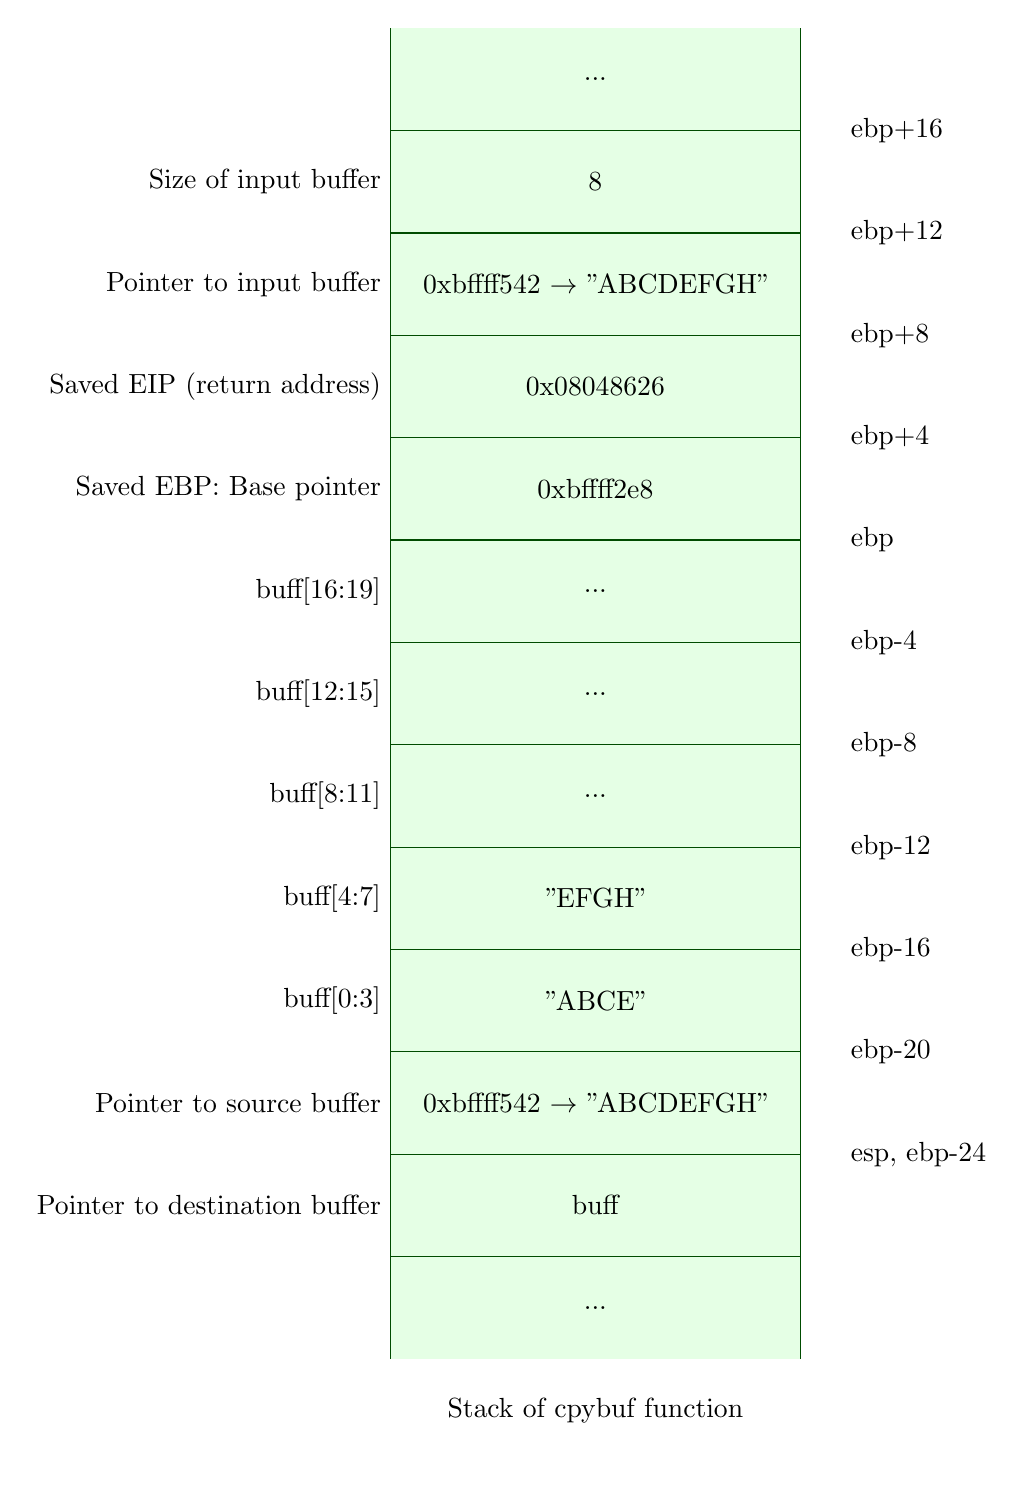
\begin{tikzpicture}[scale=1.3]
  \stacktop{}
  \cell{8} \cellcomL{Size of input buffer} \cellcom{ebp+16}
  \cell{0xbffff542 $\rightarrow$ "ABCDEFGH"} \cellcomL{Pointer to input buffer} \cellcom{ebp+12}
  \cell{0x08048626} \cellcomL{Saved EIP (return address)} \cellcom{ebp+8}
  \cell{0xbffff2e8} \cellcomL{Saved EBP: Base pointer} \cellcom{ebp+4}
  \cell{...} \cellcomL{buff[16:19]} \cellcom{ebp}
  \cell{...} \cellcomL{buff[12:15]} \cellcom{ebp-4}
  \cell{...} \cellcomL{buff[8:11]} \cellcom{ebp-8}
  \cell{"EFGH"} \cellcomL{buff[4:7]} \cellcom{ebp-12}
  \cell{"ABCE"} \cellcomL{buff[0:3]} \cellcom{ebp-16}
  \cell{0xbffff542 $\rightarrow$ "ABCDEFGH"} \cellcomL{Pointer to source buffer} \cellcom{ebp-20}
  \cell{buff} \cellcomL{Pointer to destination buffer} \cellcom{esp, ebp-24}
  \stackbottom{}
  \cell[draw=none]{Stack of cpybuf function}
\end{tikzpicture}

\end{solution}\fi

\item What is the size of the vulnerable buffer in bytes?


\ifsolution\begin{solution}
The size of vulnerable buffer is 20 bytes.

\newpage

The buffer is allocated on the stack at line \textbf{cpybuf+3}.
\begin{lstlisting}
0x804853e <cpybuf+3>      sub    esp,0x14 
...
0x804854b <cpybuf+16>     lea    eax,[ebp-0x14]
0x804854e <cpybuf+19>     push   eax
0x804854f <cpybuf+20>     call   0x80483d0 <strcpy@plt>
\end{lstlisting}

\end{solution}\fi

\end{enumerate}


\section*{Stack Buffer Overflow and Stack Overflows}
\begin{enumerate}
\item How can you exploit a stack buffer overflow to change the program flow or
run new code?  
\ifsolution
\begin{solution}
A stack buffer overflow is the result of writing more data into a buffer that was allocated on the stack. One can exploit this vulnerability to change the program flow by overwriting the return address. This address is stored on the stack at the memory location EBP+4. It can be changed to point either at the beginning of the new code (shellcode) that one intends to execute, or anywhere in the memory. Typically the shellcode is written on the stack and then the returned address is changed to point to the stack.
\end{solution}\fi


\item What is the difference between a stack buffer overflow and a stack
  overflow?
\ifsolution\begin{solution}
The \emph{stack buffer overflow} refers to the case in which a program writes beyond the end of the memory allocated on the stack for a buffer.

The \emph{stack overflow} refers particularly to the case when the execution stack grows beyond the memory that is reserved for it. For instance an endless function recursion can lead to such a vulnerability. A function recursively calls itself without termination, it will cause a stack overflow as each function call creates a new stack frame and the stack will eventually consume more memory that is reserved for it.  
\end{solution}\fi 
\end{enumerate}
%\end{enumerate}

\begin{thebibliography}{---}
\bibitem[1]{gdb}Debugging with gdb, \url{https://sourceware.org/gdb/current/onlinedocs/gdb.html}
\bibitem[2]{x86}x86 Assembly Guide, \url{http://www.cs.virginia.edu/~evans/cs216/guides/x86.html}
\bibitem[3]{stack}Stack frame layout on x86-64,  \url{http://eli.thegreenplace.net/2011/09/06/stack-frame-layout-on-x86-64/}
\bibitem[4]{vuln}Smashing The Stack For Fun And Profit,  \url{http://insecure.org/stf/smashstack.html}

\end{thebibliography}

\end{document}

